\documentclass[utf8]{gradu3}
% Jos työ on kandidaatintutkielma eikä pro gradu, käytä ylläolevan asemesta
%\documentclass[utf8,bachelor]{gradu3}
% Jos kirjoitat englanniksi, käytä ylläolevan asemesta
%\documentclass[utf8,english]{gradu3}
% tai
%\documentclass[utf8,bachelor,english]{gradu3}

\usepackage{graphicx} % kuvien mukaan ottamista varten

\usepackage{amsmath} % hyödyllinen jos tekstisi sisältää matikkaa,
                     % ei pakollinen

\usepackage{booktabs} % hyvä kauniiden taulukoiden tekemiseen

\usepackage[authordate,backend=biber,noibid]{biblatex-chicago} % biber / chicago-tyylin käyttö

\usepackage{graphicx} % kuvien lisääminen

% HUOM! Tämän tulee olla viimeinen \usepackage koko dokumentissa!
\usepackage[bookmarksopen,bookmarksnumbered,linktocpage]{hyperref}

\addbibresource{gradu_EK.bib} % Lähdetietokannan tiedostonimi

\begin{document}

\title{Vertaileva tutkimus koneoppimisen hyödyntämisestä videopelien reitinhaussa}
\translatedtitle{Comparative study of utilizing machine learning in video games' pathfinding}
\studyline{Tietotekniikka}
\tiivistelma{%
TODO: tiivistelmä suomeksi
}
\abstract{%
TODO: In english
}

\author{Emil Keränen}
\contactinformation{\texttt{emil.a.keranen@student.jyu.fi}}
% jos useita tekijöitä, anna useampi \author-komento
\supervisor{Tommi Kärkkäinen}
% jos useita ohjaajia, anna useampi \supervisor-komento
\avainsanat{koneoppiminen, videopeli, reitinhaku, syvä vahvistusoppiminen}
\keywords{machine learning, video game, pathfinding, deep reinforcement learning, Soft Actor Critic, Machine Learning Agents, Unity}

\maketitle

\bigskip

\mainmatter

\chapter{Johdanto}

- Tutkimuksen kohteena koneoppimisen tehostama reitinhaku videopeleissä
 ja sen vertaaminen heuristiseen A*-algoritmiin.

- Yleisesti reitinhaulla tarkoitetaan alku- ja loppupisteen välisen reitin selvittämistä. Useimmiten tarkoituksena
on löytää lyhin reitti väistellen samalla matkan varrella olevia esteitä.

- Reitinhakua tarvitaan videopelien lisäksi myös mm. robotiikassa. 

- Videopeleissä reitinhaku ilmenee pääasiassa tekoälyagenttien suorittamana toimintana, joten tässä tutkimuksessa keskitytään agentteihin.
Näitä agentteja kutsutaan myös ei-pelaaja-hahmoiksi (engl. non-player-character, NPC).

- Ei-pelaaja-hahmot ja itseasiassa videopelien reitinhaku vertautuvat hyvin robotiikkaan ja robottien reitinhakuun.

- Sekä robotiikassa että videopeleissä toiminta-alue voi muuttua hyvinkin paljon reaaliajassa, jolloin reitinhaun täytyy
sopeutua muutoksiin nopeasti. Käytetyt ratkaisut sen sijaan voivat vaihdella näiden kahden osa-alueen välillä: robotiikassa
tarkkuus ja turvallisuus nousevat tärkeimmiksi ominaisuuksiksi ja vastaavasti videopeleissä nopeus määrittää reitinhaun "hyvyyden".

- Reitinhaku on aina ollut vaativa ongelma videopeleissä, mutta nykyään reitinhaun ongelmallisuus voidaan
useimmissa tapauksissa sivuuttaa laatimalla heuristinen ratkaisu A*-algoritmin avulla.

- Koneoppiminen mahdollistaa aiemman kokemuksen hyödyntämisen myöhemmässä toiminnassa.
Agentteja voidaan kouluttaa harjoitteludatan avulla, jolloin ne oppivat toimimaan tuntemattomissa tilanteissa.
Koneoppimisen ansiosta reitinhaku-agentti voidaan opettaa toimimaan vaativissa ja
dynaamisissa pelialueissa, joissa muuttuvat esteet ja alueen labyrinttimäisyys
heikentävät A*-algoritmin toimintaa.

- Tutkimuksen ideana on käyttää Unity-pelimoottorille luotuja koneoppimisagentteja (engl. Unity Machine Learning Agents)
ja opettaa niitä erilaisten pelialueiden avulla. Opettamisen jälkeen agentteja testataan oikeilla
pelialueilla ja verrataan tuloksia A*-algoritmilla saatuihin tuloksiin.

- ML-agents perustuu PyTorch-kirjastoon ja mahdollistaa vahvistusoppimisen hyödyntämisen.

- Tensorboard-lisäosan avulla voidaan visualisoida palkkioiden keskiarvot ja opetuksen edistyminen opetuksen aikana.

- Pelialueiden on tarkoitus olla monimutkaisia ja dynaamisia, koska A*-algoritmi suoriutuu
yksinkertaisista reitinhakutehtävistä moitteettomasti.

\chapter{Reitinhaku videopeleissä}

Reitinhaulla tarkoitetaan yksinkertaisimmillaan reitin tai polun selvittämistä kahden pisteen välillä. Se on yksi videopelien tekoälyn ja myös robotiikan tunnetuimmista ja haastavimmista ongelmista, jota on tutkittu jo muutaman vuosikymmenen ajan \parencite{cui2011based,abd2015comprehensive}. Reitinhakua esiintyy monissa eri peligenreissä, kuten roolipeleissä ja reaaliaikaisissa strategiapeleissä, joissa ei-pelaaja-hahmoja (engl. non-player-character, NPC) määrätään liikkumaan ennaltamäärättyyn tai pelaajan määräämään sijaintiin väistellen samalla vastaantulevia esteitä. Reitinhaun ja yleisesti tekoälyn on oltava realistista, jotta pelaaja pystyy syventymään videopelin maailmaan eikä pelaajan kokema immersio keskeydy.

\section{Pelialueen esitystavat}

Pelialue esitetään reitinhakua varten aina graafina, joka koostuu solmuista ja kaarista. Kaaret yhdistävät solmut toisiinsa ja mahdollistavat liikkumisen solmujen välillä. Graafista voidaan muodostaa erilaisia kokonaisuuksia, joita kutsutaan ruudukoiksi (engl. grid). Ruudukot voivat olla kuvioltaan säännöllisiä tai epäsäännöllisiä. \parencite{lawande2022systematic}. Säännölliset ruudukot sisältävät esimerkiksi kolmioita, kuusikulmioita, neliöitä tai kuutioita riippuen onko kyseessä 2D- vai 3D-alue. Epäsäännölliset ruudukot voivat koostua esimerkiksi reittipisteistä (engl. waypoint) tai navigointiverkosta (engl. navigation mesh). Selvästi käytetyin esitystapa videopeleissä on 2D-neliöruudukko. \parencite{lawande2022systematic}.

Yleisesti ruudukot sisältävät yksittäisiä vapaita ruutuja tai esteruutuja (engl. tile). Vapaat ruudut muodostavat graafin, jolloin jokainen vapaa ruutu vastaa yhtä graafin solmuista. Vierekkäisiä ruutuja yhdistävät kaaret, joita pitkin reitinhaku ja liikkuminen tapahtuu. \parencite{botea2013pathfinding}. Solmujen vierekkäisyys voi tarkoittaa horisontaalista ja vertikaalista vierekkäisyyttä (neljä suuntaa) tai näiden lisäksi myös diagonaalista vierekkäisyyttä (kahdeksan suuntaa). \parencite{abd2015comprehensive,botea2013pathfinding}. Kuva \ref{ruudukkokuva} havainnollistaa yksinkertaista ruudukkoaluetta, jossa liikkuminen tapahtuu neljään tai kahdeksaan suuntaan.

Vaikka neliöruudukkoa pidetään tunnetuimpana ja käytetyimpänä esitystapana, se voi kuitenkin osoittautua ongelmalliseksi tilanteessa, jossa hahmo voi liikkua diagonaalisesti, jolloin kaikki vierekkäiset ruudut eivät ole saman etäisyyden päässä toisistaan. Ruudukossa, jossa ruudut ovat kooltaan 1x1, diagonaalinen etäisyys on $\sqrt{2}$, kun taas vertikaalinen tai horisontaalinen etäisyys on 1. (TODO: tähän jotain lähdettä mahdollisista ongelmista)

\begin{figure}[h]
\centering
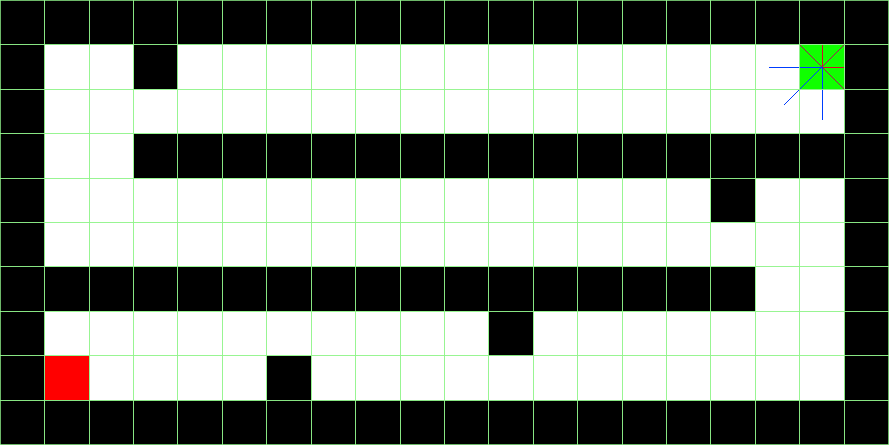
\includegraphics[width=15cm]{ruudukko_kuva.png}
\caption{Ruudukko, jossa mustat ruudut ovat esteruutuja ja valkoiset ruudut vapaita ruutuja. Vihreä ruutu on aloitusruutu ja punainen ruutu on maaliruutu.}
\label{ruudukkokuva}
\end{figure}

Vähemmän tunnettuja pelialueen esitystapoja ovat kolmiointi ja kuusikulmiointi \parencite{abd2015comprehensive}. Alueen kolmiointi ja siihen perustuvat TA*- ja TRA*-algoritmi ovat kuitenkin osoittautuneet moninkertaisesti nopeammiksi suurissa pelialueissa verrattuna A*-algoritmiin \parencite{demyen2006efficient}. Kuusikulmioihin perustuvat alueet ja reitinhakualgoritmit ovat myös tuottaneet lupaavia tuloksia robotiikan tutkimuksessa sekä yleisesti suoriutuneet paremmin muistinkäytön ja ajankäytön suhteen verrattuna neliöruudukkoihin \parencite{abd2015comprehensive,lawande2022systematic}. Epäsäännöllisistä ruudukoista navigointiverkkoa on käytetty suurimmaksi osin videopeleissä ja esimerkiksi Unity tarjoaa dokumentaatiossaan laajat ohjeet ja menetelmät navigaatioverkon luomiseen \parencite{lawande2022systematic,unitydocnavmesh}.

\section{Reitinhakualgoritmit}

Graafin lyhyimmän polun ongelmaa ja eri reitinhakualgoritmeja on tutkittu jo vuosikymmenten ajan. Vanhimmat ja tunnetuimmat algoritmit, Dijkstran algoritmi \parencite{dijkstra1959note} ja A*-algoritmi \parencite{hart1968formal}, esiteltiin jo 50- ja 60-luvuilla ja ne pystyivät ratkaisemaan lyhimmän polun ongelman staattisessa graafissa. Uudemmat reitinhaun sovellukset, kuten itseohjautuvat autot ja robotit, toivat kuitenkin alkuperäiselle ongelmanratkaisulle lisää vaatimuksia. Lyhimmän polun löytämisen lisäksi reitinhakualgoritmin täytyy ottaa huomioon sovelluksesta riippuen reitin turvallisuus, tehokkuus ja mahdollisten esteiden väistäminen \parencite{karur2021survey}.

A*-algoritmi on selvästi tunnetuin videopelien ja robottien reitinhaussa nopeutensa ansiosta \parencite{cui2011based,abd2015comprehensive,botea2013pathfinding}. A*-algoritmista on kehitetty jo monia eri variaatioita, jotka pyrkivät vastaamaan jatkuvasti kasvaviin vaatimuksiin. Tässä tutkimuksessa keskitytään tarkemmin A*-algoritmiin ja sen variaatioihin. (TODO: tähän vielä muutoksia, kuulostaa toistolta)

\subsection{A*-algoritmi}

A*-algoritmi on hyvin tunnettu paras-ensin -reitinhakualgoritmi, joka hyödyntää heuristista arviointifunktiota lyhimmän reitin etsimiseen \parencite{cui2011based,duchovn2014path}. A*-algoritmia voidaan pitää käytetyimpänä graafien etsintäalgoritmina etenkin videopeleissä \parencite{botea2013pathfinding,lawande2022systematic}.

Algoritmin toiminta tapahtuu seuraavasti: jokainen aloitussolmun vierekkäinen solmu arvioidaan kaavan \[f(n)=h(n)+g(n)\] mukaisesti, jossa \(n\) on solmu, \(h(n)\) on heuristinen etäisyys solmusta \(n\) maalisolmuun ja \(g(n)\) on todellinen etäisyys aloitussolmusta solmuun \(n\). Näistä solmuista matalimman \(f(n)\)-arvon solmu käsitellään seuraavaksi, jolloin kyseisen solmun vierekkäisten solmujen \(f(n)\)-arvot lasketaan. Tämä prosessi jatkuu, kunnes maalisolmu saavutetaan. Heuristiikan ollessa nolla A*-algoritmista tulee Dijkstran algoritmi.

A*-algoritmilla on kolme esitettyä ominaisuutta \parencite{hart1968formal}. Ensiksi A*-algoritmi löytää reitin, jos sellainen on olemassa. Toiseksi reitti on optimaalinen, jos heuristiikka on luvallinen eli arvioitu etäisyys on lyhyempi tai yhtä suuri kuin todellinen etäisyys. Viimeisenä mikään muu algoritmi samalla heuristiikalla ei käy läpi vähemmän solmuja kuin A*-algoritmi eli A* käyttää heuristiikkaa tehokkaimmalla mahdollisella tavalla. \parencite{hart1968formal,cui2011based}. Luvallisia heuristiikkoja ovat solmujen vierekkäisyydestä riippuen Euklidinen etäisyys, Manhattan-etäisyys, Chebyshev-etäisyys ja Octile-etäisyys \parencite{duchovn2014path,botea2013pathfinding}. Manhattan-etäisyyttä käytetään pääasiassa neljän suunnan ja Octile- sekä Chebyshev-etäisyyttä kahdeksan suunnan vierekkäisyyksissä \parencite{botea2013pathfinding}. Euklidista etäisyyttä voidaan käyttää tilanteessa, jossa agentti voi siirtyä seuraavaan soluun mistä kulmasta tahansa.

\subsection{A*-algoritmin variaatiot}
\label{avariaatiot}

Reitinhakualgoritmeja toteutettiin alunperin valmiisiin ja tarkkoihin ympäristöihin, joka ei kuitenkaan ole verrattavissa reaalimaailman tilanteisiin, joissa ympäristö voi muuttua arvaamattomasti \parencite{lawande2022systematic}. A*-algoritmia ja sen rajoitteita onkin tutkittu jo useita vuosikymmeniä, joka on mahdollistanut useiden eri variaatioiden kehittämisen. Useimmiten variaatiot keskittyvät korjaamaan yleisimpiä A*-algoritmin reitinhakuongelmia, kuten suoritustehon optimointia ja sopeutumista muuttuviin alueisiin \parencite{stentz1994optimal}.

Stentz (1994, 1995) esitti 90-luvulla kaksi A*-algoritmin variaatiota: D*-algoritmi (Dynamic A*) ja Focussed D*-algoritmi \parencite{stentz1994optimal,stentz1995focussed}. Uudet variaatiot pyrkivät ratkaisemaan etenkin muuttuvan ja tuntemattoman alueen ongelmat robotiikan tutkimuksessa. Alkuperäinen D*-algoritmi teki mahdolliseksi reitin korjaamisen esteen tai muutoksen tullessa reitille \parencite{stentz1994optimal}. Focussed D*-algoritmi tehosti alkuperäisen D*-algoritmin toimintaa ajallisesti ja näin ollen saattoi loppuun D*-algoritmin kehittämisprosessin \parencite{stentz1995focussed}.

Vuonna 2005 Koenig ja Likhachev (2005) esittelivät D* Lite -algoritmin, joka nimestään huolimatta ei varsinaisesti perustu suoraan D*-algoritmiin, vaan A*- ja LPA*-algoritmiin \parencite{koenig2005fast}. D* Lite -algoritmi osoittautui yksinkertaisemmaksi ja hieman tehokkaammaksi kuin D*- ja Focussed D*-algoritmit, jonka vuoksi sen toteuttaminen ja soveltaminen oli helpompaa \parencite{koenig2005fast}. (TODO: tämän kappaleen viilaus kuntoon, lainaukset, kieliasu, eteneminen jne.)

\section{Reitinhaun haasteet}

Yhden agentin staattisen ruudukkoalueen reitinhakuongelma on ratkaistavissa optimaalisesti heuristisilla reitinhakualgoritmeilla, mutta nykyään videopeleissä reitinhakuongelmat ovat monimutkaisempia ja saattavat vaatia useiden eri kriteerien täyttymisen. Suurimpia haasteita ovat esteiden järkevä väistäminen, optimaalisen reitin löytäminen ja suorituskykyvaatimusten minimointi \parencite{abd2015comprehensive,cui2011based}. Näiden lisäksi reitinhakuongelmat pitävät sisällään esimerkiksi useamman agentin samanaikaista reitinhakua ja reaaliajassa muuttuvan alueen reitinhakua. Siksi videopeleissä onkin käytössä monia eri reitinhakualgoritmeja, joista osa on kehitetty toimimaan dynaamisissa ympäristöissä, osa staattisissa ympäristöissä ja osa molemmissa \parencite{lawande2022systematic}. Reitinhakualgoritmin valinta on siis riippuvainen käyttötarkoituksesta. Nykytutkimus keskittyy pääasiassa monimutkaisten reitinhakuongelmien ratkaisemiseen ja algoritmien vertailuun erilaisissa reitinhakutilanteissa.

\subsection{Suorituskyky}

Reitinhakualgoritmin täytyy minimoida suoritustehon ja tallennustilan käyttö. Vaikka komponentit ovatkin kehittyneet vuosi vuodelta nopeasti, myös videopelit ovat monimutkaistuneet ja niiden laskennalliset vaatimukset kasvaneet. Reitinhakualgoritmeille varatut resurssit ovat videopeleissä rajatut, koska resursseja käytetään hyvin paljon myös graafisiin ja fysikaalisiin ominaisuuksiin \parencite{lawande2022systematic}. Suoritustehoon liittyen etenkin muistinkäyttöä ja laskentatehoa pidetään yleisesti rajoittavina tekijöinä videopelien reitinhaussa \parencite{botea2013pathfinding}. Ongelmia voidaan ratkaista erilaisilla algoritmeilla tai pelialueen esitystapaan liittyvillä ratkaisuilla \parencite{botea2013pathfinding,cui2011based}.

Yksi suorituskykyyn liittyvistä ongelmista on reitinhakualgoritmien huono skaalautuvuus etenkin muistinkäytön suhteen. Jos agentin reitinhakuun sovelletaan A*-algoritmia suurella 1000x1000 pelialueella, muistiin joudutaan tallentamaan jopa miljoona solmua \parencite{cui2011based,duchovn2014path}. Muistinkäyttöä havainnollistetaan kuvassa \ref{astarmemory}, jossa A*-algoritmia on käytetty esteitä sisältävän alueen reitinhakuun. Kuvan keltaiset ruudut ovat tallennettu muistiin reitinhaun aikana. Kuvasta huomaa, että A*-algoritmi käy läpi suuren määrän ylimääräisiä solmuja, koska alueella on esteitä. Ongelma moninkertaistuu, jos alueella liikkuu useita reitinhakuagentteja. Tässä tapauksessa A*-algoritmi osoittautuu riittämättömäksi ongelman ratkaisuun, joten tilanteeseen kannattaa soveltaa erilaisia menetelmiä tai algoritmien variaatioita.

TODO: tarkista vielä kuva ja sen käyttö esim. tarvitaanko? havainnollistaako tarpeeksi?

\begin{figure}[h]
\centering
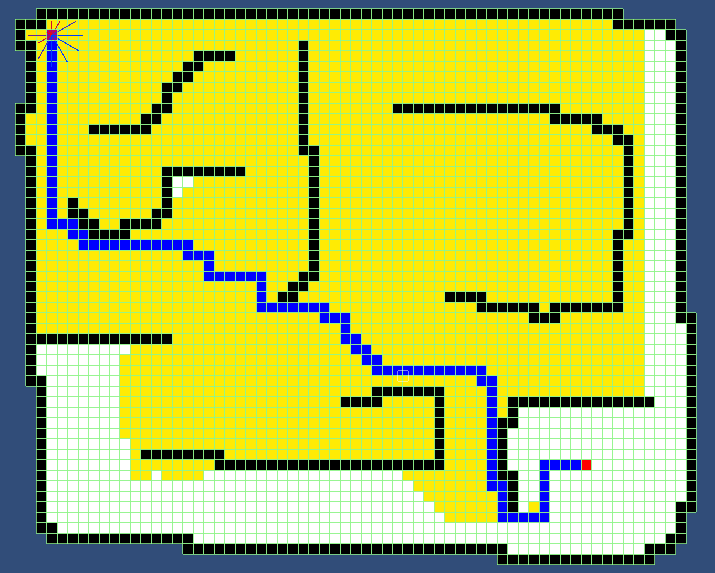
\includegraphics[width=15cm]{a_star_memory.png}
\caption{Ruudukkoalue, jossa sininen reitti on A*-algoritmin laskema optimaalisin reitti. Keltaiset ruudut ovat käsitellyt solmut, jotka on tallennettu muistiin.}
\label{astarmemory}
\end{figure}

TODO: lisää esimerkkejä, lisää suorituskykyongelmia

\subsection{Dynaamisen alueen reitinhaku}

Dynaamisen eli muuttuvan alueen reitinhaussa pyritään löytämään optimaalisin reitti jatkuvasti muuttuvassa alueessa \parencite{lawande2022systematic}. Dynaamisen alueen reitinhakua esiintyy erityisesti robotiikassa, mutta myös videopeleissä. Robottien reitinhaussa ympäröivää tilaa mitataan erilaisten sensorien avulla, jonka perusteella reitinhakua suoritetaan. Videopeleissä pelialue on kokonaisuudessaan usein valmiiksi reitinhakuagentin tiedossa eikä erillisiä sensoreita käytetä pelialueen havainnoimiseen, ellei haluta vähentää epäreiluutta ja matkia ihmismäistä käyttäytymistä. \parencite{rahmani2022towards}.

Videopeleissä pelialue voi muuttua toisten pelaajien, ei-pelaaja-hahmojen tai muuten vain liikkuvien esteiden takia. Esimerkiksi kilpa-ajoneuvopeleissä pelaaja voi kisata ei-pelaaja-hahmon kanssa, joka joutuu väistelemään sekä pelaajan ajoneuvoa että muita alueen liikkuvia esteitä \parencite{sazaki2017pathfinding}. Jokainen alueen muutos rikkoo reitinhakugraafin rakenteen, jolloin graafi ja valittu reitti täytyy korjata. Graafin luominen voi olla isoissa pelialueissa kallis operaatio, joten jatkuva uudelleenluominen ja uuden reitin etsiminen ei välttämättä ole vaihtoehto. Nykyään videopelien reitinhaun tutkimuksissa painotetaankin dynaamisia reitinhakualgoritmeja.

Graafin jatkuva päivittäminen on tuonut erilaisia ideoita tutkimuksissa. Luvussa \ref{avariaatiot} mainittu D*-algoritmi on kehitetty juuri tuntemattoman ja muuttuvan alueen reitinhakuun.

TODO: artikkeleita dynaamisesta hausta ja sen ongelmista

\subsection{Moniagenttireitinhaku}

Moniagenttireitinhaussa alueella on useampi kuin yksi agentti ja jokaisella niistä on oma aloitus- ja lopetuspisteensä graafissa. Jokaisella aika-askeleella agentti voi joko liikkua toiseen solmuun tai pysyä paikallaan nykyisessä solmussaan. \parencite{sharon2015conflict,stern2019multi}. Tarkoituksena on samaan aikaan ratkaista moniagenttireitinhakuongelma ja minimoida reitinhaun kustannusfunktio (engl. cost function). Yleinen kustannusfunktio on \textit{sum-of-costs}, joka on agenttien aika-askelten summa kun ne saapuvat kohteisiinsa. Kustannusfunktiona voi olla myös \textit{makespan}, joka minimoi ajan kunnes viimeinen agentti on saapunut kohdesolmuun tai \textit{fuel}, joka minimoi agenttien kulkeman matkan. Erityisenä huomiona fuel-kustannusfunktiossa on se, että paikallaan odottaminen ei nosta kustannuksia. \parencite{sharon2015conflict}.

Moniagenttireitinhaun rajoitteet voivat vaihdella tutkimusalasta riippuen, kuten esimerkiksi saavatko agentit kulkea samaa reittiä pitkin seuraten toisiaan, mutta yleensä perusrajoitteet ovat samat \parencite{sharon2015conflict,stern2019multi}. Perinteisesti agenttien täytyy liikkua lopetuspisteeseen törmäämättä toisiinsa matkalla ts. yhdellä solmulla ei saa olla samanaikaisesti enempää kuin yksi agentti. Kaksi agenttia eivät myöskään saa kulkea saman kaaren kautta samalla aika-askeleella. Moniagenttireitinhakuongelman sovelluksia esiintyy videopelien lisäksi esimerkiksi robotiikassa, ilmailussa, liikennesuunnittelussa ja itseohjautuvissa ajoneuvoissa, joten se on saanut viime vuosina paljon huomiota tutkimuksissa ja akateemisissa yhteisöissä. \parencite{sharon2015conflict,stern2019multi}.

Moniagenttireitinhakuongelmaan on sekä optimaalisia että epäoptimaalisia ratkaisuja. Optimaaliset ratkaisut ovat luonteeltaan NP-kovia, koska agenttien lukumäärä kasvattaa ongelman tila-avaruutta eksponentiaalisesti. A*-algoritmi on esimerkiksi optimaalinen ratkaisu, mutta moniagenttireitinhaussa sen suoritusaika voi olla hyvin pitkä ja muistinkäyttö liian suurta. \parencite{sharon2015conflict}. Tämän vuoksi ongelmissa, joissa agentien lukumäärä on suuri, käytetään usein epäoptimaalisia ratkaisuja. 

TODO: moniagenttireitinhaku oikea termi?

\chapter{Koneoppiminen}

Koneoppiminen on tällä hetkellä yksi teknisten tutkimusalojen suosituimmista aihealueista. Sen ydin rakentuu kysymykselle, pystyykö tietokone jäljittelemään ihmismielen oppimisprosessia ja täten oppia automaattisesti kokemuksen kautta. \parencite{das2017survey,jordan2015machine}. Automaattisella oppimisella pyritään vähentämään manuaalista, tapaus tapauksen perään ohjelmoimista. Sen sijaan konetta opetetaan syöte-tuloste -parien avulla. Vuosikymmenten aikana koneoppimisen tutkimus on edistynyt hyvin paljon eikä loppua ole toistaiseksi näkymässä. Uudet sovellukset ja algoritmit, laskentatehon kasvu ja big data eli hyvin suuret, keskittyneet datamäärät ovat tuoneet tarpeen sekä teorian tutkimukselle että kehittyneille käytännön ratkaisuille.

\section{Koneoppimisen perusteet}

Koneoppiminen on tieteenalana yhdistelmä tietotekniikkaa ja tilastotieteitä. Tietotekniikka ja tietokoneet mahdollistavat ongelmanratkaisun. Suurista datajoukoista oppiminen, erilaisten ennusteiden tekeminen ja päätöksenteko vaativat sen sijaan tilastotieteellisiä menetelmiä. \parencite{das2017survey,jordan2015machine}. Myös neurotieteiden ja psykologian roolit ovat kasvamassa koneoppimisen tutkimuksessa. Esimerkiksi ihmisaivojen ja sitä kautta oppimisprosessin tutkiminen ja hyödyntäminen koneoppimisessa ovat tulevaisuudessa merkittäviä tutkimuksen kohteita. \parencite{das2017survey}. Koneoppimisen sovellukset ovat nykyään hyvin laaja-alaiset. Tunnettuja esimerkkejä ovat konenäkö, puheentunnistus ja robotiikka. Konenäköä hyödynnetään etenkin terveydenhoidon alalla anomalioiden tunnistamiseen kuvissa. Mainonnassa koneoppimista käytetään personoitujen suositusten luomiseen ja markkinoinnissa erilaisissa ennusteissa.

Tietoteknisten laitteiden suosio ja sitä kautta datan räjähdysmäinen kasvu ovat olleet suuressa roolissa koneoppimisen hyödyntämisessä. Kyseisiä suuria datamassoja eli big dataa on mahdotonta tarkastella manuaalisesti, joten niiden käsittelyyn on otettu käyttöön koneoppimisen menetelmiä. Koneoppimisalgoritmit pystyvät muokkaamaan palveluita vastaamaan jokaisen henkilökohtaisiin tarpeisiin personoidun datan avulla. Esimerkiksi mainoksia voidaan kohdentaa tietyille ryhmille ja vanhoja potilastietoja voidaan hyödyntää hoitotyypin valitsemiseen tietyille potilaille. \parencite{jordan2015machine}. Personoitu data tuo tosin tietoturvallisia haasteita. Henkilödatasta on pyrittävä tekemään anonyymia, jottei sitä pysty yhdistämään suoraan henkilöihin. Samalla kuitenkin data voi olla niin tarkkaa, että jokaisella sanotaan olevan oma digitaalinen sormenjälki suuressa datamassassa. Myös suorituskykyvaatimukset ovat nousseet datan kasvun myötä, joten algoritmit täytyy kehittää mukautuviksi \parencite{jordan2015machine}.

Koneoppimisella yritetään perinteisesti ratkaista luokitteluongelmia, joissa datajoukosta voidaan päätellä, kuuluuko käsiteltävä asia tiettyyn luokkaan vai ei \parencite{jordan2015machine}. Esimerkiksi sähköposti voidaan luokitella roskapostiksi tai aidoksi sähköpostiksi riippuen mitkä ovat luokittelun vaihtoehdot. Koneoppimisen avulla kasvatetaan luokittelun tarkkuutta, joka on kyseisen luokitteluongelman tärkein mittari. Esimerkkidata, jolla konetta opetetaan, voi koostua kokoelmasta erilaisia sähköposteja, jotka on valmiiksi luokiteltu roskapostiksi tai aidoksi sähköpostiksi. Syötteenä on siis sähköposti ja tulosteena "roskaposti" tai "aito". Koneoppimisen avulla kone opetetaan tunnistamaan malleja ja kuvioita datassa, jolloin se pystyy myöhemmin tunnistamaan samoja kuvioita oikeissa tilanteissa. \parencite{jordan2015machine}.

\section{Koneoppimisen paradigmat}

Koneoppiminen voidaan jakaa eri osiin oppimistyylin mukaan. Oppimistyylejä ovat esimerkiksi ohjattu oppiminen, puoliohjattu oppiminen, ohjaamaton oppiminen, transduktio ja vahvistusoppiminen \parencite{das2017survey}. Näistä tunnetuimpia ovat ohjattu oppiminen, ohjaamaton oppiminen ja vahvistusoppiminen.

\subsection{Ohjattu oppiminen}

Käytetyin oppimistyyli on ohjattu oppiminen ja siihen liittyvät menetelmät \parencite{jordan2015machine}. Ohjatussa oppimisessa oppiminen tapahtuu luokitellun aineiston perusteella. Se havainnollistaa lineaariapproksimaatiota ja siihen liittyviä ongelmia. Opetusaineisto tuodaan \((x,y)\) pareina, jossa \(x\) on syöte, esimerkiksi kuva, ja \(y\) on tulos, esimerkiksi lintu. Oppijan tavoitteena on tuottaa mahdollisimman tarkka ennuste \(y\) syötteen \(x\) perusteella. \parencite{jordan2015machine}.

Ohjatun oppimisen heikkoutena voidaan pitää luokitellun datan saatavuutta \parencite{das2017survey}. Data täytyy esikäsitellä ja luokitella ennalta muilla menetelmillä, joka nostaa lopullista laskentakustannusta.

TODO: hieman niukka kappale, mahdollisesti lisää tekstiä.

\subsection{Ohjaamaton oppiminen}

Ohjaamattomassa oppimisessa analysoidaan luokittelematonta dataa \parencite{das2017survey,jordan2015machine}. Tarkoituksena on tehdä päätelmiä datan rakenteesta ja malleista ilman ulkopuolista ohjeistusta. Klusterointi ja dimension redusointimenetelmät ovat yleisiä datan strukturointimenetelmiä (mikä muu termi tähän sopisi?).

Klusteroinniksi kutsutaan menetelmiä, joissa datapisteet jaetaan ominaispiirteidensä perusteella klustereihin. Yksittäiset klusterit sisältävät siis ominaisuuksiltaan samankaltaiset datapisteet. \textit{K-means} -klusterointi on tunnettu klusterointimenetelmä, jossa datapisteet \(n\) jaetaan \(K\):hon klusteriin. Klusterin keskipistettä lähimpänä oleva datapiste toimii eräänlaisena prototyyppinä, johon muiden datapisteiden etäisyyksiä verrataan. Uusi datapiste katsotaan kuuluneeksi siihen klusteriin, jonka keskipisteeseen on pienin etäisyys.

Dimension redusointimenetelmät pyrkivät tihentämään datajoukkoa ja helpottamaan sen analysointia. Niiden periaatteena on vähentää datajoukossa tarkasteltavia ominaispiirteitä ja näin ollen vähentää datajoukon kokonaisulottuvuutta, jolloin datajoukon analysointi yksinkertaistuu. Uuteen datajoukkoon pyritään sisällyttämään keskeisimmät piirteet siten, ettei relevanttia informaatiota katoaisi. Pääkomponenttianalyysi on yksi tunnetuimmista ja vanhimmista dimension redusointimenetelmistä, jossa olemassaolevasta datajoukosta poimitaan tärkeimmät piirteet ja luodaan niistä pääkomponentteja (engl. principal components) \parencite{abdi2010principal}.

\subsection{Vahvistusoppiminen}

Vahvistusoppiminen on kolmas suuri koneoppimisen paradigma, jossa oppijana toimii agentti ja agentin toimintaa ohjaavat palkkiot \parencite{jordan2015machine}. Vahvistusoppimisen harjoitusdata eroaa muiden paradigmojen harjoitusdatasta siten, ettei tietylle syötteelle \(x\) anneta valmiiksi oikeaa tulosta \(y\) tai etsitä rakenteellisia malleja datajoukosta, vaan agentti saa jokaisesta suorittamastaan toiminnosta positiivisen tai negatiivisen palkkion \parencite{jordan2015machine}. Palkkiot ohjaavat agentin oppimisprosessia ja käyttäytymistä ympäristössä. Toimintojen ja niistä saatujen palkkioiden lisäksi agentti on jatkuvassa vuorovaikutuksessa ympäristönsä kanssa siten, että agentti tarkkailee toimintojensa vaikutuksia ja ympäristön tilamuutoksia. Näin agentti pystyy muokkaamaan toimintojaan saamiensa palkkioiden perusteella. \parencite{arulkumaran2017brief}. Vahvistusoppimistehtävän ideaaliratkaisu on palkkiot maksimoivan käytännön (engl. policy) selvittäminen.

Vahvistusoppiminen voidaan kuvata Markovin päätösprosessina (engl. Markov decision process, MDP) tilojen \(S\), toimintojen \(A\) ja palkkiosignaalien \(r\) avulla. Jokaisella aika-askeleella \(t\) agentti suorittaa toiminnon \(a\), jolloin ympäristön tila \(s\) muuttuu ja muutos viestitään agentille palkkiosignaalin \(r\) kautta. Palkkiosignaalin lisäksi ympäristö viestii agentille tilamuutoksesta, jolloin agentti saa tiedon uudesta tilasta \(s\) + 1. Palkkion ja uuden tilan perusteella agentti valitsee jälleen seuraavan toimintonsa. Agentin lopullisena tavoitteena on saavuttaa paras mahdollinen käytäntö (engl. policy), joka maksimoi saadun palkkion määrän. Kuva \ref{reinflearning} havainnollistaa vahvistusoppimisen toimintaa.

\begin{figure}[h]
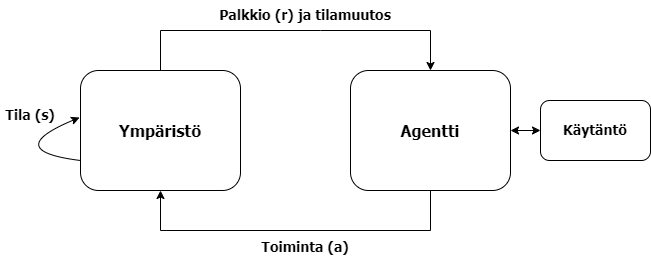
\includegraphics[width=15cm]{reinflearning.png}
\caption{Vahvistusoppimisympäristön oppimissilmukka yhdellä aika-askeleella.}
\label{reinflearning}
\end{figure}

Oppiakseen optimaalisen käytännön agentin tekemät päätökset vaativat jonkin ennusteen tulevien toimintojen arvosta. Yleisesti tämän ennusteen laskemista kutsutaan nimellä \textit{action-value function}, ja yksi tunnettu menetelmä sen laskemiseen on Q-oppiminen (engl. Q-learning). Q-oppiminen on malliton (engl. model-free) menetelmä eli se ei tarvitse toimiakseen erillistä mallia ympäristöstä. Q-oppimisessa jokaisen tilan eri toimintoa arvioidaan \cite{arulkumaran2017brief} esittämän kaavan \[Q(s,a) = r_t + \gamma max_a Q^\pi (s_{t+1},a)\] mukaisesti, jossa \(s\) on tila, \(a\) on toiminto, \(r_t\) on tilan palkkio, $\gamma$ on erillinen vähennys, joka määrittelee tulevien toimintojen tärkeyden aiempiin verrattuna ja \(max_a Q^\pi (s_{t+1},a)\) on ennakkoarvio tulevasta, optimaalisesta palkkiosta.

TODO: tarkista vielä q-oppimiseen liittyvät asiat

Funktiosta saatuja arvoja päivitetään erillisessä Q-taulussa. Oppimisepisodien aikana agentti pystyy ennakoimaan Q-taulun avulla jokaisen mahdollisen toimintonsa tulevaa lopullista palkkiota ja tarvittaessa päivittämään Q-taulun arvoja. Ongelmaksi osoittautuu kuitenkin uuden tutkimisen (engl. exploration) ja olemassa olevan tiedon hyödyntämisen (engl. exploitation) tasapainotus \parencite{arulkumaran2017brief}. \textit{Epsilon-Greedy} on menetelmä, jossa tietyllä todennäköisyydellä $\epsilon$ agentti valitsee pienemmän arvon tilan, jolloin voidaan löytää uusia, parempia ratkaisuja haluttuun lopputulokseen. Agentti voi myös jatkaa aiemman käytännön hyödyntämistä todennäköisyydellä 1 - $\epsilon$.

Vahvistusoppimiseen liittyy haasteita optimaalisen käytännön löytämisessä ja agentin satunnaisissa toiminnoissa \parencite{arulkumaran2017brief}. Optimaalinen käytäntö on mahdollista löytää vain jatkuvan yrittämisen kautta, ja ainoana oppimisen signaalina toimivat saadut palkkiot. Riippuen tehtävän haastavuudesta lukuisatkaan yritykset eivät välttämättä takaa optimaalisinta ratkaisua. Toiseksi agentin palkkioon johtavissa toiminnoissa saattaa olla paljon turhia toimintoja eli toisin sanoen agentti ei välttämättä tiedä, mitkä toiminnot oikeasti johtivat palkkion saamiseen. Esimerkiksi robotin liikkuessa sisätiloissa sen havainnot riippuvat vahvasti siitä, kohtaako se matkalla umpikujia vai siirtyykö se satunnaisilla toiminnoilla suoraan kohteeseen. Jos palkkio annetaan maaliin pääsyn yhteydessä, niin robotti olettaa, että umpikujaan päätyminen kuului palkkion saamiseen vaativien toimintojen joukkoon. Tätä ongelmaa kutsutaan nimellä \textit{(temporal) credit assignment problem}.

\section{Syväoppiminen}

Koneoppimisen ja sitä kautta myös syväoppimisen tutkimus on ollut viime vuosina hyvin aktiivista \parencite{pouyanfar2018survey}. Syväoppimisella ollaan onnistuttu ratkaisemaan ongelmia, joita tekoälyn tutkimuksessa on yritetty ratkaista vuosia \parencite{lecun2015deep,pouyanfar2018survey}. Erityisesti tuloksia on tullut kuvantunnistuksessa, puheentunnistuksessa ja erilaisissa luonnollisen kielen prosessoinnin tehtävissä \parencite{lecun2015deep,pouyanfar2018survey}. Suurimpia syväoppimisen tutkimuksen askeleita viime vuosikymmenillä ovat vastavirta-algoritmi (engl. backpropagation), konvoluutioneuroverkon (engl. Convolutional Neural Network, CNN) inspiraationa tunnettu neocogitron-neuroverkko, siitä hieman myöhemmin kehitetty takaisinkytketty neuroverkko (engl. Recurrent Neural Network, RNN) ja syvä uskomusverkko (engl. Deep Belief Network, DBM). Syvä uskomusverkko mahdollisti entistä syvemmän neuroverkon oppimisen, jonka seurauksena siirryttiin yleisesti käyttämään termiä syväoppiminen. Viime vuosien yksi tunnetuimpia syväoppimisen sovelluksia on muun muassa Googlen AlphaGo, joka onnistui päihittämään useita Go-pelin ammattilaisia pelin äärimmäisestä strategisesta haastavuudesta huolimatta. Tässä luvussa kerrotaan neuroverkkojen, syväoppimisen ja syvän vahvistusoppimisen toiminnan perusteet sekä esitellään Soft Actor Critic -algoritmi, jota myöhemmin sovelletaan tutkimuksen empiirisessä osuudessa.

\subsection{Neuroverkkojen perusteet}

Neuroverkkojen perusosiin kuuluvat perseptronit (engl. perceptron), jotka ovat keinotekoisia neuroneita \parencite{nielsen2015neural}. Perseptronit koostuvat binäärisistä syötteistä \(x_{1}, x_{2}, x_{3},..,\) ja yksittäisestä binäärisestä tuloksesta. Syötteiden relevanttius määritellään erillisten painoarvojen (engl. weight) \(w_{1}, w_{2}, w_{3},..,\) perusteella. Syötteet ja painoarvot lasketaan painotettuna summana $\sum_{j}w_{j}x_{j}$ ja tulokseen lisätään neuronin vakiotermi (engl. threshold tai bias), joka on neuronille parametrina annettu luku ja määrittää onko lopullisena tuloksena 0 vai 1. Yksinkertaistettuna \cite{nielsen2015neural} kuvaa perseptronia "laitteeksi, joka tekee päätökset punnitsemalla todisteita".

Yleisesti neuroverkko koostuu syötekerroksesta, piilokerroksesta ja ulostulokerroksesta \parencite{nielsen2015neural}. Piilokerros koostuu yhdestä tai useammasta perseptroni-kerroksesta. Ensimmäisellä perseptroni-kerroksella tehdään yksinkertaisimmat päätökset ja jokaisella seuraavalla kerroksella tehdään toinen toistaan monimutkaisempia päätöksiä. Kerrosten suuri lukumäärä mahdollistaa siis vaativienkin päätösten tekemisen.

Oppiminen on mahdollista painoarvoja muuttamalla, jolloin koko neuroverkon lopullinen tulos muuttuu \parencite{nielsen2015neural}. Vaarana kuitenkin on, että pienet muutokset muuttavat neuroverkon tulosta radikaalisti vastakkaiseen suuntaan. Korvaamalla alkuperäiset, binääriset perseptronit Sigmoid-neuroneilla painoarvojen muutokset eivät aiheuta suurta muutosta tuloksessa. Sigmoid-neuronit käyttävät sigmoid-funktiota porrasfunktion sijaan, jolloin tulos voi olla mitä tahansa 0 ja 1 välillä.

Kuten koneoppimisessa, myös syväoppimisessa neuroverkon opettaminen tapahtuu harjoitusdatan avulla \parencite{nielsen2015neural}. Luokitteluongelman suoran ratkaisemisen sijaan neuroverkon opettamisessa keskitytään ensin painoarvojen ja vakiotermien muodostaman virhefunktion minimiarvon löytämiseen ja vasta sen jälkeen luokittelun tarkkuuteen. Virhefunktion minimin löytämiseen käytetään tunnettua optimointikeinoa, gradienttimenetelmää (engl. gradient descent) ja vastavirta-algoritmia (engl. backpropagation). Vastavirta-algoritmilla voidaan laskea kerralla gradianttimenetelmään tarvittavat osittaisderivaatat painoarvojen ja vakiotermien suhteen virhefunktiossa. Tuloksena saadaan virhefunktion gradientti, jonka jälkeen painoarvot ja vakiotermit päivitetään neuroneissa takaperin iteroiden viimeisestä kerroksesta lähtien ja menetelmä toistetaan.

Gradienttimenetelmällä pyritään yleisellä tasolla selvittämään virhefunktion minimi suorittamalla pieniä askeleita kohti globaalia tai lokaalia minimiä \parencite{nielsen2015neural}. Askeleiden pituus määritellään oppimisnopeudella (engl. learning rate), joka on usein pieni vakioluku. Oppimisnopeus ei saa kuitenkaan olla liian pieni, koska muuten algoritmi toimii hyvin hitaasti. Oppimisnopeutta voidaan tehostaa myös käyttämällä stokastista gradienttimenetelmää, jossa painoarvot ja vakiotermit päivitetään vasta pienen harjoitusdatajoukon jälkeen. Tästä saatu tulos toimii hyvänä arviona todelliselle gradienttivektorille.

\subsection{Syväoppimisen haasteet}

Yksi suurimmista syväoppimisen haasteista on ylisovittaminen (engl. overfitting) \parencite{nielsen2015neural}. Ylisovittamisessa neuroverkko oppii harjoitusdatan liiankin täsmällisesti ja menettää sen johdosta kykynsä yleistää oppimaansa toisiin tapauksiin esimerkiksi testiesimerkkidatassa. Ylisovittamista ilmenee usein jos harjoitusdatan luokittelun tarkkuus nousee lähelle sataa prosenttia, mutta testiesimerkkidatan luokittelun tarkkuus pysyy ennallaan. Ylisovittamista voidaan estää esimerkiksi neuroverkon pienentämisellä tai harjoitusdatan kasvattamisella. Joskus opettaminen voidaan myös keskeyttää, jos testiesimerkkidatan tarkkuus ei tunnu enää kasvavan.

Ylisovittamista voidaan hillitä myös säännöstelyllä (engl. regularization), jossa pyritään pienentämään neuronien painoarvoja virhefunktion minimin löytämiseen \parencite{nielsen2015neural}. Suurten painoarvojen pienet muutokset voivat aiheuttaa suuria muutoksia neuroverkon toimintaan, jolloin se voi ajautua ylisovittamaan harjoitusdataa. Säännöstely toisin sanoen tehostaa neuroverkon kykyä tehdä yleistyksiä. Yleisiä säännöstelymenetelmiä ovat L1- ja L2-säännöstelyt sekä neuronien poistaminen (engl. dropout). Neuronien poistaminen eroaa muista mainituista siten, ettei siinä keskitytä virhefunktion muokkaamiseen, vaan neuroverkon piilokerroksesta poistetaan hetkellisesti neuroneita. Neuroverkon toiminta pysyy muuten ennallaan, mutta vain osaa neuroneista käytetään ja niiden parametreja päivitetään. Seuraavalla iteraatiolla neuronit palautetaan ja jälleen osa piilokerroksen neuroneista poistetaan väliaikaisesti. (Jokainen iteraatio käyttää opettamiseen rakenteeltaan erilaista neuroverkkoa, koska osa neuroneista on piilotettu. Tämän avulla saadaan luotua tilanne, jossa samaa neuroverkkoa opettaessa opetetaankin useita erilaisia neuroverkkoja ja näiden neuroverkkojen ylisovittamiset kumoavat toisensa.)

TODO: Tarkista neuroverkkoteorian sisältö, onko riittävä?

\section{Syvä vahvistusoppiminen}

Yksi tekoälyn tutkimuksen suurimpia tavoitteita on luoda täysin autonominen ja ohjailtava agentti, joka pystyy toimimaan erilaisissa ympäristöissä samalla oppien ja kehittäen käyttäytymistään paremmaksi \parencite{arulkumaran2017brief}. Alunperin vahvistusoppimisella pystyttiin kehittämään oppivia agentteja, mutta ongelmaksi osoittautui ongelmien ja ratkaisujen suppeus, koska pelkällä vahvistusoppimisella ei pystytty käsittelemään ja hyödyntämään moniulotteista dataa, kuten robotin raakaa sensoridataa tai kuvan pikseleitä. Syväoppimisella onnistuttiin vastaamaan tähän vaatimukseen, ja pian syvän vahvistusoppimisen sovelluksilla pystyttiin jo pelaamaan Atari 2600:n videopelejä käyttämällä hyväksi kuvan pikselidataa.

\subsection{Syvän vahvistusoppimisen perusteet}

Syvä vahvistusoppiminen hyödyntää syväoppimista ja neuroverkkoja suurten tila- ja havaintoavaruuksien vahvistusoppimistapauksissa \parencite{li2018deep}. Se eroaa vahvistusoppimisesta pääasiassa funktioapproksimaation suhteen. Esimerkiksi tavallisessa Q-oppimisessa muodostetaan taulu tila-toiminta -pareista ja niiden Q-arvoista, mutta syvässä Q-oppimisessa (engl. deep Q-learning) taulu korvataan neuroverkolla. Syvässä Q-oppimisessa tila, esimerkiksi pikselidata, syötetään neuroverkolle ja tuloksena saadaan mahdolliset toiminnot ja niiden arvot. Oppiminen tapahtuu neuroverkon tapaisesti eli selvitetään funktion maksimiarvot ja päivitetään neuroverkon painoarvoja sen mukaisesti.

TODO: policy search, experience replay, bootstrapping..

\subsection{Soft actor-critic}

Soft actor-aritic (SAC) on \cite{haarnoja2018soft} kehittämä malliton (oikea termi?) ja \textit{off-policy} syvä vahvistusoppimis-algoritmi. Se kehitettiin vastaamaan yleisiin vahvistusoppimis-algoritmien ongelmiin reaalimaailmassa, kuten harjoitusdatan kompleksisuuteen (engl. sample complexity) ja hyperparametrien herkkyyteen \parencite{haarnoja2018app}. Yksinkertaisetkin tehtävät saattoivat vaatia satoja tuhansia ellei jopa miljoonia opetusaskeleita ennen kuin sopiva lopputulos saavutettiin. Tämän lisäksi eri tehtävien välillä joutui virittelemään monien eri hyperparametrien arvoja, jotta oppiminen olisi edes mahdollista. SAC pyrkii mahdollisimman satunnaisiin toimintoihin samalla maksimoiden odotetun palkkiomäärän, jota kutsutaan myös nimellä \textit{maximum entropy}. Tavallisesti parhaimman käytännön löytämisessä halutaan maksimoida saatu palkkio, mutta \textit{maximum entropy} -periaatteessa yhtälöön lisätään erillinen entropia-termi. Entropian suuruutta kontrolloidaan erillisen kertoimen $\alpha$ avulla, joka voidaan asettaa myös nollaksi, jolloin yhtälö palauttaa jälleen maksimipalkkion antavan käytännön.

TODO: SAC testauksesta, suoriutui paremmin kuin muut DRL-algoritmit, ehkä lisää teoriataustaa?

\chapter{Unity}

Unity on Unity Technologiesin kehittämä pelinkehitysalusta, joka sisältää oman renderöinti- ja fysiikkamoottorin sekä Unity Editor -nimisen graafisen käyttöliittymän \parencite{juliani2018unity}. Unityllä on mahdollista kehittää perinteisten 3D- ja 2D-pelien lisäksi myös esimerkiksi VR-pelejä tietokoneille, mobiililaitteille ja pelikonsoleille. Unitystä onkin vuosien mittaan tullut yksi tunnetuimmista pelinkehitysalustoista, jonka parissa työskentelee kuukausittain jopa 1.5 miljoonaa aktiivista käyttäjää \parencite{unityweb}.

Viime vuosina Unityä on käytetty simulointialustana tekoälytutkimuksen parissa. Unity mahdollistaa lähes mielivaltaisten tilanteiden ja ympäristöjen simuloinnin 2D ruudukkokartoista monimutkaisiin pulmanratkaisutehtäviin, joka on sen suurimpia vahvuuksia simulointialustana. Kehitystyö ja prototypointi ovat Unityllä myös erityisen nopeaa. \parencite{juliani2018unity}.

\section{Unityn hierarkia}

Tässä luvussa käsitellään Unityn hierarkiaa. Aliluvuissa käydään läpi hierarkian osat ylimmästä lähtien.

\subsection{Unity-projekti}

Unityn hierarkian ylin osa on projekti, jonka luomisesta kehitystyö aina alkaa. Unityssä on mahdollista luoda projekti valmiista pohjista, joita ovat esimerkiksi 2D-, 3D- ja VR-pohjat. Pohjien avulla projekteihin saa lisättyä suoraan suositeltavat, parhaita käytäntöjä mukailevat asetukset.

Unity-projekteja voidaan hallinnoida ja avata erillisellä Unity Hub -sovelluksella. Unity Hub kertoo muun muassa mitä Unityn versiota projekti tukee. Projekteja voi tarvittaessa siirtää (engl. migrate) toimimaan uusimmilla Unityn versioilla, mutta siirto voi aiheuttaa toiminnallisuuksien muutoksia tai virheitä projektissa.

\subsection{Näkymät}

Projektista seuraavana hierarkiassa ovat näkymät (engl. scene). Näkymät toimivat työskentelyalustoina projektissa. Projekti sisältää aina yhden tai useamman näkymän, koska ilman niitä mitään ei pysty luomaan. Tavallisesti yksittäinen näkymä kuvaa aina yhtä kenttää, tasoa tai aluetta pelissä, ja siirryttäessä toiselle alueelle Unity pystyy lataamaan ajon aikana uuden skenen. Näkymän lataaminen voi tosin viedä aikaa, joten lataus peitetään useimmiten latausruuduilla, jotka voivat myös olla omia, yksinkertaisia näkymiä. Yksinkertaisimmillaan peli voi kuitenkin sisältää vain yhden näkymän, joka muokkautuu ja jota muokataan ajon aikana.

Projektin luonnin jälkeen Unity lisää siihen automaattisesti aloitusnäkymän, joka sisältää kamera- ja valonlähde-peliobjektin. Tätä näkymää voi lähteä muokkaamaan lisäämällä siihen erilaisia peliobjekteja, esimerkiksi maata ja erilaisia geometrisia muotoja.

\subsection{Peliobjektit ja Prefabit}

Peliobjektit (engl. GameObject) ovat tärkein osa Unityn pelinkehitysprosessia, koska kaikki peliin luotavat objektit ovat taustaltaan peliobjekteja. Peliobjektit eivät itsessään tee mitään tai näytä miltään, vaan ne toimivat säiliöinä komponenteille. Peliobjekteja voidaan järjestellä vanhempi-lapsi -periaatteella. Lapsiobjektit liikkuvat vanhemman mukana, jolloin niitä ei tarvitse liikutella näkymässä erikseen. Kuva \ref{peliobjektikuva} havainnollistaa esimerkkinäkymän peliobjekteja ja niiden vanhempi-lapsi -suhteita.

Prefabit ovat peliobjektien valmiita malleja, joita luodaan peliobjektien tavoin. Prefabit vähentävät toistuvaa työtä peliobjektien luomisen yhteydessä. Prefabeille voidaan lisätä komponentteja ja lapsiobjekteja kuten peliobjekteille. Kun prefabi lisätään näkymään, sen komponentteja ja arvoja voidaan muuttaa tarvittaessa ilman, että alkuperäisen prefabin arvot ja komponentit muuttuvat.

Peliobjekteja voi lisätä "GameObject"-valikosta Unityn ylävalikosta joko tyhjinä objekteina tai valmiina kokonaisuuksina. Valmiita peliobjekteja ovat esimerkiksi erilaiset valonlähteet tai 3D-objektit, ja ne sisältävät automaattisesti tarvittavat komponentit.

\begin{figure}[h]
\centering
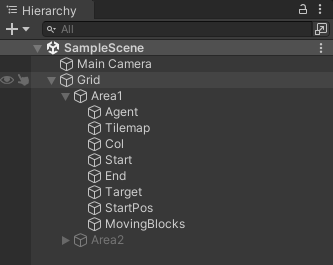
\includegraphics[width=8.8cm]{peliobjektilistaus.png}
\caption{Lista peliobjekteista avoimessa näkymässä. Sisäkkäiset peliobjektit ovat lapsiobjekteja.}
\label{peliobjektikuva}
\end{figure}

\subsection{Komponentit}

Komponentit antavat peliobjekteille ominaisuuksia ja toiminnallisuuksia kuten muodon, värin tai fysiikan. Komponentteja voi olla rajattomasti, mutta peliobjektilla on luonnin jälkeen vähintään Transform-komponentti, joka määrittää peliobjektin sijainnin, suunnan ja skaalan. Transform-komponenttia ei voi poistaa peliobjektilta. Esimerkiksi valmis 3D-objekti pallo (sphere) saa automaattisesti Mesh Filter-, Mesh Renderer- ja Sphere Collider-komponentit. Kaksi ensimmäistä komponenttia keskittyvät pallon graafisiin ominaisuuksiin ja Sphere Collider fyysisiin törmäysominaisuuksiin. Sphere Collider-komponentti asettuu automaattisesti pallon graafisen ulkomuodon kokoiseksi.

Usein komponenteilla on erilaisia arvoja, kuten koko tai väri, joita voi muokata käyttöliittymäelementtien avulla. Komponentit voivat sisältää myös viittauksia muihin peliobjekteihin, tiedostoihin tai assetteihin(käännös?). Esimerkiksi Sprite Renderer -komponenttiin voidaan lisätä viittaus kuvatiedostoon, jolloin Unity renderöi peliobjektin kohdalle lisätyn kuvan. Kuvassa \ref{komponenttikuva} on lista peliobjektin komponenteista ja 

\begin{figure}[t]
\centering
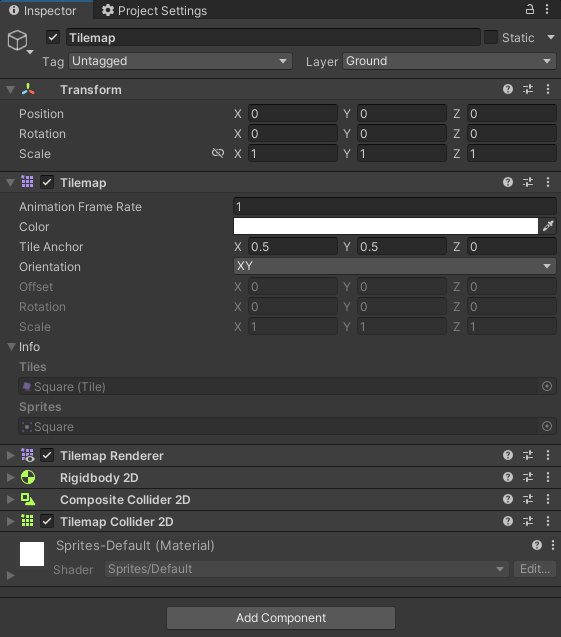
\includegraphics[width=14.8cm]{komponenttilistaus.png}
\caption{Lista peliobjektin komponenteista.}
\label{komponenttikuva}
\end{figure}

\subsection{Skriptit}

Ohjelmoinnin merkitys Unityn käytössä tulee skripteistä. Skriptit ovat ohjelmakooditiedostoja, joita voi lisätä peliobjektiin komponentin tavoin, jos valmiit komponentit eivät riitä toiminnallisuuksiltaan. Skripteissä voi esimerkiksi määritellä ominaisuuksia ja arvoja, joita voi muokata komponenttilistauksessa tai ajon aikana. Unity tukee tällä hetkellä vain C-\# -ohjelmointikieltä, mutta ennen myös Javascriptiin pohjautuvaa UnityScript-ohjelmointikieltä.

Unity tarjoaa skripteihin MonoBehaviour-pohjaluokan, joka mahdollistaa pelinkehityksen tärkeimmät osat eli Start()-aloitusfunktion ja Update()-päivitysfunktion. Start()-funktio ajetaan ennen yhtäkään päivitysfunktiota, joten siinä voidaan määrittää ja alustaa tarvittavat alkuarvot. Update()-funktio ajetaan joka ruudunpäivityskerralla, joten siihen sijoitetaan usein pelilogiikka ja mahdollisesti fyysiset toiminnallisuudet.

Skriptien avulla voidaan tehdä lähes kaikki samat asiat kuin Unity Editorissa. Peliobjekteja voidaan etsiä tagien tai nimien kautta ja niille voidaan lisätä ja poistaa komponentteja ajon aikana. Käyttämättömät peliobjektit voidaan tuhota tai asettaa epäaktiivisiksi jos niitä ei tarvita.

\section{Machine Learning Agents}

Machine Learning Agents on Unitylle kehitetty ilmainen koneoppimispaketti, joka mahdollistaa Unity Editorilla luotujen simulaatioympäristöjen ja Python APIn välisen vuorovaikutuksen. ML-Agents SDK (Software Development Kit) tarjoaa kaikki toiminnallisuudet ja skriptit toimivan koneoppimisympäristön luomiseen. \parencite{juliani2018unity}. Kuva \ref{mlagentsstructure} havainnollistaa Unity Editorilla luodun yksinkertaisen ML-Agents koneoppimisympäristön toimintaa. TODO: "unity editorilla luodun" vai pelkästään "ML-agentsin toimintaa/rakennetta"

\subsection{ML-Agents SDK}

ML-Agents SDK sisältää kolme ydinosaa: sensorit, agentit ja akatemia. Agentti-komponentti voidaan lisätä suoraan Unityn peliobjektille, jolloin se pystyy keräämään havaintoja, suorittamaan toimintoja ja vastaanottamaan palkkioita. Sensorit mahdollistavat havaintojen keräämisen eri tavoin. Akatemia ylläpitää tietoa simulaation askelmäärästä ja ympäristön parametreista sekä ohjaa agenttien toimintaa.

\begin{figure}[h]
\centering
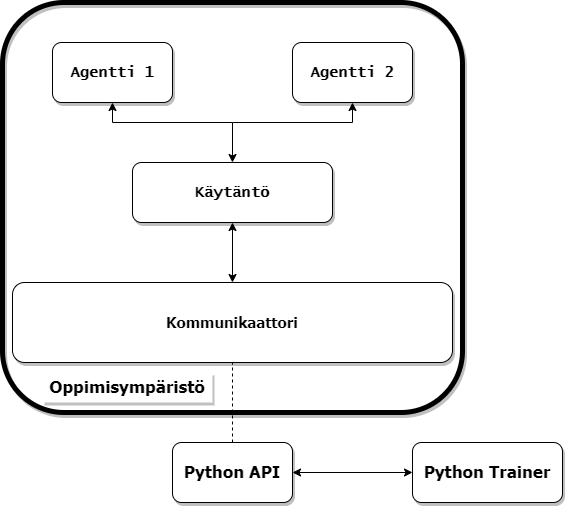
\includegraphics[width=15cm]{mlagents_structure.png}
\caption{Lohkokaavio Unity ML-Agents toiminnasta.}
\label{mlagentsstructure}
\end{figure}

Agentin käytäntö määritellään Behavior Name -nimikkeen avulla. Eri agenteilla voi olla sama käytäntö, jolloin agentit käyttävät kyseistä käytäntöä päätöksentekoon ja jakavat harjoitteludatan keskenään. Myös useiden erilaisten agenttien toiminta voidaan mahdollistaa erinimisillä käytännöillä.

\subsection{Python API ja PyTorch}

Python APIa käytetään Unityllä tehdyn simulaatioympäristön ja koneoppimissilmukan käsittelyyn. APIn avulla tekijän ei tarvitse itse olla suoraan yhteydessä Pythonin koneoppimiskouluttajaan, vaan API tarjoaa helppokäyttöiset, valmiit menetelmät koneoppimissilmukan luomiseen. Tarkemmin APIsta ja sen toiminnasta voi lukea dokumentaatiosta (tähän linkki sivun alalaitaan tulevasta docsista?).

PyTorch on avoimen lähdekoodin koneoppimiskehys, johon pohjautuen Unity ML-agents -paketin koneoppimiseen liittyvät toteutukset on tehty (Unity ML agents docs). PyTorch sisältää kaikki syvän koneoppimisen perusosat datan kanssa työskentelystä ja koneoppimismallin luomisesta mallin parametrien optimointiin ja oppimismallien tallentamiseen (PyTorch docs).

\chapter{Tutkimuksen empiirinen osuus}

Tässä kappaleessa käsitellään tutkimuksen empiiristä osuutta. Tutkimus toteutettiin empiirisenä vertailevana tutkimuksena. Vertailun kohteena olivat Unityn ML-agentin suorittama reitinhaku ja heuristiseen A*-algoritmiin perustuva reitinhaku. Kappaleessa \ref{sec:tutkimuksenkuvaus} kuvaillaan tutkimusta yleisellä tasolla ja esitellään tutkimuksessa käytetyt työkalut. Kappaleessa \ref{sec:tutkimusasetelma} käydään läpi simulaatioympäristöt ja koneoppimiseen liittyvät konfiguraatiot. Lopuksi kappaleessa \ref{sec:mittaaminen} käsitellään tulosten mittaamista ja käytettyjä suureita.

\section{Tutkimuksen kuvaus}
\label{sec:tutkimuksenkuvaus}

Tutkimuksen simulaatioalustana käytettiin Unityä, koska sen käyttö oli ennestään tuttua ja se soveltuu hyvin erilaisten tilanteiden simuloimiseen. Unity mahdollisti valmiit menetelmät ruudukkoalueen toteutukseen, jolloin ympäristön luomiseen ei mennyt liikaa aikaa. Tutkimusta varten luotiin valmis 2D-projekti ja projektiin lisättiin Unity Package Managerin avulla ML-Agents -paketti, jotta tarvittavat toiminnallisuudet saatiin käyttöön koneoppimista varten. Unityllä luotiin yksinkertaisia ruudukkoalueita, jonne sijoitettiin esteruutuja, kävelykelpoisia ruutuja ja alku- ja loppuruudut sekä joissain alueissa liikkuvia esteitä. Reitinhaun vertailua varten luotiin A*-algoritmi ja erikseen opetettiin koneoppimisagentti. Koneoppimisagentti käyttää syvään vahvistettuun oppimiseen perustuvaa SAC-algoritmia.

A*-algoritmia täytyi muokata tutkimukseen sopivaksi. Pelialueet ovat dynaamisia eli muuttuvat reaaliaikaisesti, joten perinteinen A*-algoritmi ei pysty reagoimaan muutoksiin välittömästi. Algoritmia muokattiin tutkimukseen siten, että esteen ilmestyessä laskelmoidulle reitille A*-algoritmi ajetaan uudestaan, mutta lähtöpisteeksi asetetaan agentin uusi sijainti. Uusi sijainti on agentin siihen asti etenemä matka, jolloin seuraava reitinhakuiteraatio vaatii lyhyemmän matkan. Jokainen iteraatio on myös suurimmassa osassa tapauksista kevyempiä muistinkäytön kannalta.

\section{Tutkimusasetelma / Konfiguraatio}
\label{sec:tutkimusasetelma}

Koneoppimisagentin toiminta riippuu vahvasti sen asetuksista.

- AddObservation()-funktion avulla agentti kerää tietoa omasta tilastaan ympäristössä. Tässä tutkimuksessa agentin täytyy kerätä tietoa sen omasta sijainnista (x ja y), mahdollisesti etäisyydestä maaliin (toimisiko esim. laskea manhattan-etäisyys?) ja maalin sijainnista (x ja y). Suositeltavaa kuitenkin on, että agentti keräisi tietoa vain näkemistään asioista eli tässä tapauksessa vain omasta sijainnistaan. Näiden havaintojen lisäksi käytetään RayPerceptionSensor2D-komponenttia, joka kerää ympäröivästä alueesta tietoa säteiden avulla. Tässä projektissa agentista lähetetään 12 sädettä, jotka yltävät vain yhden ruudun verran eteenpäin. Säteet pystyvät tunnistamaan vastaantulevia objekteja, joita ovat tässä tapauksessa esteet ja maaliruutu. Näiden havaintojen avulla agentti voi tehostaa päätöksentekoaan.

- Actions, toiminnat, yksinkertaisen pelialueen takia käytetään Discrete Actions ja viittä eri vaihtoehtoa (ylös, alas, oikealle, vasemmalle, paikallaan). Jos pelialue olisi monimutkaisempi, voidaan käyttää Continuous Actions (suunta + nopeus).

- Rewards, palkinnot, agentti saa positiivisen palkkion kun saapuu maaliin (+1). Agentti saa negatiivisen palkkion jokaisen toiminnan (action) jälkeen (-0.01). Jos agentti törmäilee seiniin, eli yrittää liikkua suuntaan jossa on este, agentille annetaan negatiivinen palkkio (-0.001). Palkkiot määritellään skriptitiedostossa ja ovat helposti muutettavissa.

- Agentin opettaminen aloitetaan komentoriviltä komennolla ml-agents "BehaviorName"... (myös jotain muuta, ml-agents -komento hyödyntää siis Python APIa). Komentorivi näyttää käyttäjän asettamien opetusaskelten välein mm. agentin keskiarvopalkkion askelten aikana. Tässä tutkimuksessa asetettiin väliksi 10000, tensorboard päivittyy myös 10000 välein ts. piirtää kuvaajan pisteen?

\section{Tulosten mittaaminen}
\label{sec:mittaaminen}

- Reitinhakutehtävästä otetaan talteen aika (sekuntia) ja onnistuiko reitinhaku vai ei (onnistui/epäonnistui).

\chapter{Tulokset ja johtopäätökset}

\chapter{Yhteenveto}

\printbibliography

\chapter{Liitteet}

- Kuvat tai mallinnokset pelialueesta.

- Tensorboardin kuvaajat mm. agentin palkkioiden kehityksestä.

\end{document}
